\documentclass[10pt,aspectratio=169]{beamer}

\usetheme{Madrid}
\setbeamertemplate{navigation symbols}{}
\setbeamertemplate{footline}[frame number]

\usepackage[utf8]{inputenc}
\usepackage[T1]{fontenc}
\usepackage[french]{babel}
\usepackage{amsmath,amssymb}
\usepackage{booktabs}
\usepackage{array}
\usepackage{graphicx}
\usepackage{tikz}
\usepackage{listings}
\usepackage{xcolor}
\usetikzlibrary{arrows.meta,positioning,fit,calc,shapes.geometric}

\graphicspath{{../docs/}{../slides/fig/}{assets/}}

\definecolor{adcBlue}{RGB}{18,64,114}
\definecolor{adcInk}{RGB}{25,30,38}
\definecolor{adcGray}{RGB}{86,94,108}
\definecolor{adcLight}{RGB}{240,243,247}
\definecolor{adcGreen}{RGB}{34,132,86}
\definecolor{adcOrange}{RGB}{195,108,40}
\definecolor{adcRed}{RGB}{166,55,64}
\definecolor{codeBg}{RGB}{247,248,250}

\setbeamercolor{title}{fg=adcBlue}
\setbeamercolor{frametitle}{fg=white,bg=adcBlue}
\setbeamercolor{structure}{fg=adcBlue}
\setbeamercolor{normal text}{fg=adcInk}
\setbeamercolor{block title}{fg=white,bg=adcBlue}
\setbeamercolor{block body}{bg=adcLight,fg=adcInk}

\lstdefinestyle{cppslide}{
  language=C++,
  basicstyle=\ttfamily\fontsize{5.6}{6.3}\selectfont,
  keywordstyle=\color{adcBlue}\bfseries,
  commentstyle=\color{adcGreen},
  stringstyle=\color{adcOrange},
  columns=fullflexible,
  keepspaces=true,
  showstringspaces=false,
  backgroundcolor=\color{codeBg},
  frame=single,
  rulecolor=\color{adcLight},
  breaklines=true,
  morekeywords={concept,requires,constexpr,ADC_HD,Real,KOKKOS_LAMBDA}
}
\lstdefinestyle{bashslide}{
  language=bash,
  basicstyle=\ttfamily\fontsize{5.8}{6.5}\selectfont,
  keywordstyle=\color{adcBlue}\bfseries,
  columns=fullflexible,
  keepspaces=true,
  showstringspaces=false,
  backgroundcolor=\color{codeBg},
  frame=single,
  rulecolor=\color{adcLight},
  breaklines=true
}

\newcommand{\code}[1]{\texttt{\footnotesize #1}}
\newcommand{\src}[1]{{\scriptsize\color{adcGray}Source : \texttt{\footnotesize\detokenize{#1}}}}
\newcommand{\eqbox}[1]{\begin{beamercolorbox}[wd=\textwidth,sep=0.35cm,rounded=true]{block body}#1\end{beamercolorbox}}
\newcolumntype{L}[1]{>{\raggedright\arraybackslash}p{#1}}

\title[\texttt{adc\_cpp}]{\texttt{adc\_cpp} : architecture d'un solveur hyperbolique--elliptique AMR}
\subtitle{Abstraction C++, solveurs, AMR, MPI/GPU, résultats ROMEO}
\author{Romain Despoulain}
\institute{Présentation tuteur}
\date{\today}

\begin{document}

\begin{frame}[plain]
  \vspace{0.35cm}
  {\Large\bfseries\color{adcBlue}\texttt{adc\_cpp} : architecture d'un solveur hyperbolique--elliptique AMR}

  \vspace{0.25cm}
  {\large Abstraction C++, solveurs, AMR, MPI/GPU, résultats ROMEO}

  \vspace{0.45cm}
  \[
    \frac{\partial U}{\partial t}+\nabla\!\cdot F(U,\mathrm{aux})=S(U,\mathrm{aux}),
    \qquad
    \mathcal{D}\phi=f(U),\qquad
    \mathrm{aux}=(\phi,\nabla\phi)
  \]

  \vspace{0.25cm}
  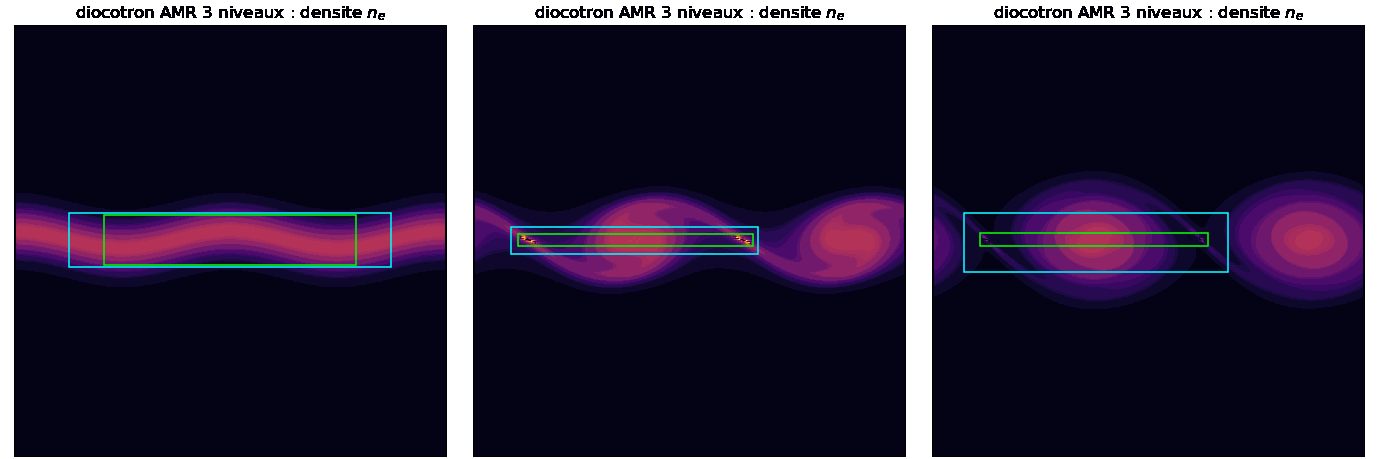
\includegraphics[width=\textwidth,height=0.26\textheight,keepaspectratio]{romeo_amr3_sequence.png}

  \vfill
  {\small Romain Despoulain \hfill \today}
\end{frame}

\section{Modèle abstrait}

\begin{frame}{Problème discret ciblé}
  \eqbox{
  \[
    \partial_t U+\nabla\!\cdot F(U,\mathrm{aux})=S(U,\mathrm{aux}),
    \qquad
    \mathcal{D}\phi=f(U),\qquad
    \mathrm{aux}=(\phi,\nabla\phi)
  \]
  }

  \vspace{0.25cm}
  \begin{columns}[T,onlytextwidth]
    \begin{column}{0.49\textwidth}
      \textbf{Partie hyperbolique}
      \begin{itemize}
        \item volumes finis cartésiens ;
        \item flux numérique Rusanov, HLL, HLLC ;
        \item reconstruction NoSlope, MUSCL, WENO5-Z ;
        \item intégration SSP-RK / IMEX / splitting.
      \end{itemize}
    \end{column}
    \begin{column}{0.49\textwidth}
      \textbf{Partie elliptique}
      \begin{itemize}
        \item multigrille géométrique 5 points ;
        \item FFT périodique mono-rang ou distribuée ;
        \item champ auxiliaire dérivé par différences centrées ;
        \item couplage par étage ou une fois par pas.
      \end{itemize}
    \end{column}
  \end{columns}

  \vspace{0.15cm}
  \src{include/adc/operator/spatial_operator.hpp, include/adc/elliptic/}
\end{frame}

\begin{frame}{Domaine de validité du contrat}
  \begin{columns}[T,onlytextwidth]
    \begin{column}{0.51\textwidth}
      \textbf{Ce que le contrat couvre}
      \begin{itemize}
        \item systèmes conservatifs ou quasi conservatifs ;
        \item flux et sources locaux, évaluables cellule par cellule ;
        \item fermeture elliptique de type Poisson ou opérateur analogue ;
        \item champ auxiliaire utilisé dans le flux ou dans la source.
      \end{itemize}
    \end{column}
    \begin{column}{0.45\textwidth}
      \textbf{Exemples déjà présents}
      \begin{itemize}
        \item diocotron : \(\mathrm{aux}\rightarrow F\) ;
        \item Euler--Poisson : \(\mathrm{aux}\rightarrow S\) ;
        \item deux-fluides AP : source raide traitée par intégrateur dédié.
      \end{itemize}
    \end{column}
  \end{columns}

  \vspace{0.35cm}
  \begin{block}{Limite explicite}
    Un modèle cinétique, non local ou multi-elliptique ne rentre pas seulement par
    \code{PhysicalModel}. Il faut alors introduire un opérateur discret plus riche.
  \end{block}
\end{frame}

\begin{frame}[fragile]{Contrat C++ : \texttt{PhysicalModel}}
\begin{lstlisting}[style=cppslide]
template <class M>
concept PhysicalModel =
  requires(const M m, const typename M::State u,
           const typename M::Aux a, int dir) {
    typename M::State;
    typename M::Aux;
    { M::n_vars } -> std::convertible_to<int>;
    { m.flux(u, a, dir) } -> std::same_as<typename M::State>;
    { m.max_wave_speed(u, a, dir) } -> std::convertible_to<Real>;
    { m.source(u, a) } -> std::same_as<typename M::State>;
    { m.elliptic_rhs(u) } -> std::convertible_to<Real>;
  };
\end{lstlisting}
  \src{include/adc/core/physical_model.hpp}

  \vspace{0.2cm}
  \begin{itemize}
    \item Le modèle physique fournit seulement des formules ponctuelles.
    \item Il ne voit ni \code{MultiFab}, ni MPI, ni AMR, ni Kokkos.
    \item Les types \code{State} et \code{Aux} sont compatibles host/device.
  \end{itemize}
\end{frame}

\begin{frame}[fragile]{Exemple réel : modèle diocotron}
\begin{lstlisting}[style=cppslide]
struct Diocotron {
  using State = StateVec<1>;
  using Aux = adc::Aux;
  static constexpr int n_vars = 1;

  Real B0 = 1.0;
  Real n_i0 = 1.0;
  Real alpha = 1.0;

  ADC_HD Real drift_velocity(const Aux& a, int dir) const {
    return (dir == 0) ? (-a.grad_y / B0) : (a.grad_x / B0);
  }
  ADC_HD State flux(const State& u, const Aux& a, int dir) const {
    State f{};
    f[0] = u[0] * drift_velocity(a, dir);
    return f;
  }
  ADC_HD Real max_wave_speed(const State&, const Aux& a, int dir) const {
    const Real d = drift_velocity(a, dir);
    return d < 0 ? -d : d;
  }
  ADC_HD State source(const State&, const Aux&) const { return State{}; }
  ADC_HD Real elliptic_rhs(const State& u) const {
    return alpha * (u[0] - n_i0);
  }
};
\end{lstlisting}
  \src{include/adc/model/diocotron.hpp}
\end{frame}

\begin{frame}{Deux usages de \(\mathrm{aux}\)}
  \begin{columns}[T,onlytextwidth]
    \begin{column}{0.49\textwidth}
      \begin{block}{Diocotron : \(\mathrm{aux}\) dans le flux}
        \[
          \partial_t n_e+\nabla\!\cdot(n_e \mathbf{v}_E)=0,
          \qquad
          \mathbf{v}_E=\frac{1}{B_0}
          \begin{pmatrix}
            -\partial_y\phi\\
             \partial_x\phi
          \end{pmatrix}
        \]
        \[
          \Delta\phi=\alpha(n_e-n_{i0})
        \]
      \end{block}
    \end{column}
    \begin{column}{0.49\textwidth}
      \begin{block}{Euler--Poisson : \(\mathrm{aux}\) dans la source}
        \[
          \partial_t U+\nabla\!\cdot F_{\rm Euler}(U)=S(U,\nabla\phi)
        \]
        \[
          S=(0,\rho g_x,\rho g_y,\rho\mathbf{u}\!\cdot\!\mathbf{g}),
          \qquad
          \mathbf{g}=-\nabla\phi
        \]
      \end{block}
    \end{column}
  \end{columns}

  \vspace{0.25cm}
  Un même \code{assemble\_rhs} assemble \(R=-\nabla\cdot F+S\) ; seul le modèle change.
\end{frame}

\section{Architecture}

\begin{frame}{Architecture du dépôt}
  \begin{center}
  \begin{tikzpicture}[
    node distance=0.32cm,
    layer/.style={draw,rounded corners=2pt,minimum width=10.7cm,minimum height=0.70cm,align=center,fill=adcLight},
    arrow/.style={-{Latex[length=2.5mm]},thick,adcBlue}
  ]
    \node[layer,fill=adcBlue!13] (phys) {\textbf{Physique} : \code{core/physical\_model.hpp}, \code{model/}};
    \node[layer,below=of phys] (num) {\textbf{Numérique} : \code{operator/}, \code{elliptic/}};
    \node[layer,below=of num] (data) {\textbf{Données} : \code{mesh/box\_array.hpp}, \code{mesh/multifab.hpp}, \code{amr/}};
    \node[layer,below=of data] (exec) {\textbf{Exécution} : \code{mesh/for\_each.hpp}, \code{parallel/comm.hpp}, \code{core/allocator.hpp}};
    \node[layer,below=of exec] (time) {\textbf{Temps/couplage} : \code{integrator/}, \code{coupling/}};
    \draw[arrow] (phys) -- (num);
    \draw[arrow] (num) -- (data);
    \draw[arrow] (data) -- (exec);
    \draw[arrow] (exec) -- (time);
  \end{tikzpicture}
  \end{center}

  \vspace{0.15cm}
  \begin{block}{Point architectural}
    Les conteneurs décrivent où sont les données. Les frontières d'exécution décrivent
    comment on parcourt ou communique. Les deux ne sont pas mélangés.
  \end{block}
\end{frame}

\begin{frame}{Carte des modules principaux}
  \small
  \begin{tabular}{@{}p{0.22\textwidth}p{0.72\textwidth}@{}}
  \toprule
  \textbf{Module} & \textbf{Rôle dans le solveur} \\
  \midrule
  \code{core/} & \code{Real}, \code{ADC\_HD}, \code{StateVec}, \code{Aux}, concept \code{PhysicalModel}. \\
  \code{model/} & Diocotron, Euler, Euler--Poisson, deux-fluides isotherme, Langmuir. \\
  \code{operator/} & Reconstructions, flux numériques, \code{assemble\_rhs}, flux de face pour reflux. \\
  \code{elliptic/} & \code{EllipticSolver}, multigrille géométrique, FFT Poisson. \\
  \code{mesh/} & \code{Box2D}, \code{BoxArray}, \code{DistributionMapping}, \code{Fab2D}, \code{MultiFab}. \\
  \code{integrator/} & SSP-RK, IMEX, splitting, moteur AMR \code{advance\_amr}. \\
  \code{coupling/} & \code{Coupler}, \code{AmrCouplerMP}, regrid, diagnostics AMR. \\
  \code{solver/}, \code{src/} & façades compilées \code{libadc} pour applications et bindings Python. \\
  \bottomrule
  \end{tabular}
\end{frame}

\begin{frame}{Boucle de couplage hyperbolique--elliptique}
  \begin{center}
  \begin{tikzpicture}[
    cstage/.style={draw,rounded corners=2pt,minimum width=3.3cm,minimum height=0.78cm,align=center,fill=adcLight},
    arrow/.style={-{Latex[length=2.5mm]},thick,adcBlue},
    node distance=0.65cm and 0.85cm
  ]
    \node[cstage] (u) {\(U^n\)};
    \node[cstage,right=of u] (rhs) {\(f(U)\)\\\code{elliptic\_rhs}};
    \node[cstage,right=of rhs] (phi) {\(\mathcal D\phi=f\)\\MG ou FFT};
    \node[cstage,below=of phi] (aux) {\(\mathrm{aux}=(\phi,\nabla\phi)\)};
    \node[cstage,left=of aux] (res) {\(R=-\nabla\cdot F+S\)\\\code{assemble\_rhs}};
    \node[cstage,left=of res] (rk) {SSP-RK\\\(U^{n+1}\)};
    \draw[arrow] (u) -- (rhs);
    \draw[arrow] (rhs) -- (phi);
    \draw[arrow] (phi) -- (aux);
    \draw[arrow] (aux) -- (res);
    \draw[arrow] (res) -- (rk);
    \draw[arrow] (rk) -- ++(-0.45,0) |- (u);
  \end{tikzpicture}
  \end{center}

  \vspace{0.2cm}
  \begin{itemize}
    \item \code{PerStageCoupling} : Poisson résolu à chaque étage RK.
    \item \code{OncePerStepCoupling} : champ gelé pendant le pas, plus rapide mais ordre de couplage plus faible.
  \end{itemize}
\end{frame}

\begin{frame}[fragile]{Code réel : \texttt{Coupler::advance}}
\begin{lstlisting}[style=cppslide]
template <class Limiter = NoSlope, class Policy = PerStageCoupling>
void advance(MultiFab& U, Real dt) {
  MultiFab R(ba_, dm_, Model::n_vars, 0);

  update_aux(U);                         // Poisson -> phi -> aux
  fill_ghosts(U, geom_.domain, bcU_);
  assemble_rhs<Limiter>(model_, U, aux_, geom_, R);
  MultiFab U1 = U;
  saxpy(U1, dt, R);

  if constexpr (std::is_same_v<Policy, PerStageCoupling>)
    update_aux(U1);                      // champ recalcule au 2e stage
  fill_ghosts(U1, geom_.domain, bcU_);
  assemble_rhs<Limiter>(model_, U1, aux_, geom_, R);
  saxpy(U1, dt, R);
  lincomb(U, Real(0.5), U, Real(0.5), U1);
}
\end{lstlisting}
  \src{include/adc/coupling/coupler.hpp}
\end{frame}

\begin{frame}{Discrétisation hyperbolique}
  \begin{columns}[T,onlytextwidth]
    \begin{column}{0.48\textwidth}
      \textbf{Flux de face}
      \[
        \widehat F=
        \frac12\big(F(U_L)+F(U_R)\big)
        -\frac12\alpha(U_R-U_L)
      \]
      \[
        \alpha=\max\lambda(U_L,U_R,\mathrm{aux})
      \]
      \begin{itemize}
        \item Rusanov par défaut ;
        \item HLL/HLLC pour Euler ;
        \item flux de face conservés pour le reflux AMR.
      \end{itemize}
    \end{column}
    \begin{column}{0.48\textwidth}
      \textbf{Reconstruction}
      \begin{itemize}
        \item \code{NoSlope} : ordre 1, robuste ;
        \item \code{Minmod}, \code{VanLeer}, \code{MC} : MUSCL ordre 2 ;
        \item \code{WENO5Z} : ordre 5 pour convergence diocotron.
      \end{itemize}
      \vspace{0.2cm}
      \includegraphics[width=\linewidth,height=0.32\textheight,keepaspectratio]{fig_diocotron_highorder.png}
    \end{column}
  \end{columns}
\end{frame}

\begin{frame}{Solveur elliptique}
  \begin{columns}[T,onlytextwidth]
    \begin{column}{0.50\textwidth}
      \textbf{\code{EllipticSolver}}
      \begin{itemize}
        \item \code{rhs()} : second membre \(f(U)\) ;
        \item \code{phi()} : solution conservée en warm start ;
        \item \code{solve()} : inversion ;
        \item \code{residual()} : contrôle numérique.
      \end{itemize}
      \vspace{0.2cm}
      \src{include/adc/elliptic/elliptic_solver.hpp}
    \end{column}
    \begin{column}{0.46\textwidth}
      \textbf{Backends présents}
      \begin{itemize}
        \item \code{GeometricMG} : V-cycle Gauss--Seidel rouge/noir, compatible AMR.
        \item \code{PoissonFFTSolver} : direct, périodique, mono-rang.
        \item \code{DistributedFFTSolver} : bandes MPI, \code{MPI\_Alltoall}.
      \end{itemize}
      \vspace{0.2cm}
      \includegraphics[width=\linewidth,height=0.28\textheight,keepaspectratio]{tut_poisson_backends.png}
    \end{column}
  \end{columns}
\end{frame}

\begin{frame}{Solveurs physiques implémentés}
  \scriptsize
  \begin{tabular}{@{}L{0.20\textwidth}L{0.42\textwidth}L{0.30\textwidth}@{}}
  \toprule
  \textbf{Solveur} & \textbf{Équation} & \textbf{Validation} \\
  \midrule
  \code{Diocotron} &
  transport \(E\times B\), Poisson sur \(n_e-n_{i0}\) &
  croissance linéaire ; invariants ; AMR. \\
  \code{Euler} &
  Euler compressible 2D &
  Sod ; vortex isentropique. \\
  \code{EulerPoisson} &
  Euler + force \(-\nabla\phi\), signe gravité/plasma &
  Jeans ; Bohm--Gross. \\
  \code{TwoFluidAP} &
  deux-fluides isotherme asymptotic-preserving &
  limite raide ; dispersion ; cyclotron. \\
  \bottomrule
  \end{tabular}

  \vspace{0.35cm}
  \normalsize
  \begin{block}{Frontière bibliothèque}
    \code{solver/} et \code{src/} fournissent des façades compilées
    non templatisées. Le coeur générique reste dans \code{include/adc/}.
  \end{block}
\end{frame}

\section{AMR}

\begin{frame}{AMR block-structured}
  \begin{columns}[T,onlytextwidth]
    \begin{column}{0.48\textwidth}
      \textbf{Objets}
      \begin{itemize}
        \item \code{BoxArray} : liste globale des patchs ;
        \item \code{DistributionMapping} : patch \(\rightarrow\) rang ;
        \item \code{MultiFab} : champ distribué par patchs ;
        \item \code{AmrLevelMP} : \(U\), \(\mathrm{aux}\), \(\Delta x\), \(\Delta y\).
      \end{itemize}
      \vspace{0.15cm}
      \textbf{Invariants}
      \begin{itemize}
        \item ratio 2 entre niveaux ;
        \item sous-cyclage temporel Berger--Oliger ;
        \item reflux aux interfaces coarse--fine.
      \end{itemize}
    \end{column}
    \begin{column}{0.48\textwidth}
      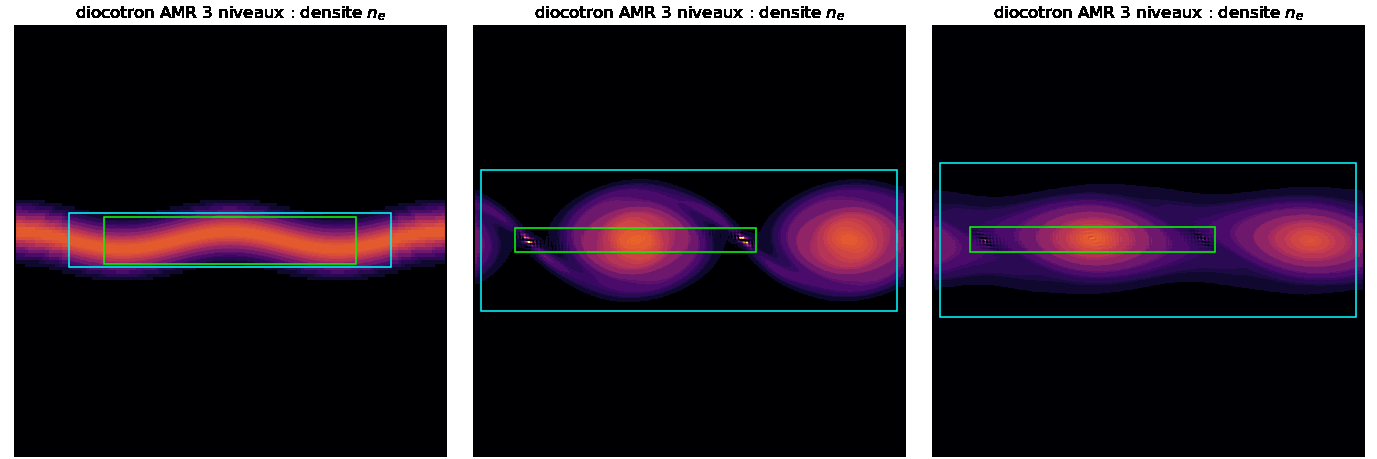
\includegraphics[width=\linewidth]{diocotron_amr3_sequence.png}

      \vspace{0.15cm}
      {\scriptsize Diocotron AMR 3 niveaux, frames extraites de \code{docs/anim\_diocotron\_amr3.gif}.}
    \end{column}
  \end{columns}
\end{frame}

\begin{frame}{Pas AMR conservatif}
  \begin{center}
  \begin{tikzpicture}[
    box/.style={draw,rounded corners=2pt,fill=adcLight,minimum width=2.65cm,minimum height=0.62cm,align=center,font=\scriptsize},
    arrow/.style={-{Latex[length=2.2mm]},thick,adcBlue},
    node distance=0.55cm and 0.42cm
  ]
    \node[box] (sync) {average-down\\fin \(\to\) grossier};
    \node[box,right=of sync] (poisson) {Poisson grossier\\\(\phi\)};
    \node[box,right=of poisson] (inject) {injection\\\(\mathrm{aux}\)};
    \node[box,below=of inject] (coarse) {avance grossier\\\(\Delta t\)};
    \node[box,left=of coarse] (fine) {avance fin\\\(r\) sous-pas};
    \node[box,left=of fine] (reflux) {reflux\\flux fin - flux grossier};
    \node[box,below=of fine] (regrid) {regrid\\tags + Berger--Rigoutsos};
    \draw[arrow] (sync) -- (poisson);
    \draw[arrow] (poisson) -- (inject);
    \draw[arrow] (inject) -- (coarse);
    \draw[arrow] (coarse) -- (fine);
    \draw[arrow] (fine) -- (reflux);
    \draw[arrow] (reflux) -- ++(-0.35,0) |- (sync);
    \draw[arrow,dashed] (fine) -- (regrid);
    \draw[arrow,dashed] (regrid) -| (sync);
  \end{tikzpicture}
  \end{center}

  \vspace{0.25cm}
  \begin{itemize}
    \item \code{compute\_face\_fluxes} expose les flux nécessaires au reflux.
    \item \code{CoverageMask} évite de corriger les interfaces fin--fin.
    \item \code{FluxRegister} agrège average-down et reflux, y compris sous MPI.
  \end{itemize}
\end{frame}

\begin{frame}[fragile]{Code réel : entrée AMR de production}
\begin{lstlisting}[style=cppslide]
void step(Real dt) {
  update();  // sync_down + Poisson + grad(phi) + injection aux
  advance_amr<NoSlope, RusanovFlux>(
      model_, stack_.L(), stack_.domain(), dt,
      Periodicity{true, true}, replicated_coarse_);
}

template <class Crit>
void regrid(Crit crit, int grow = 2, int margin = 2) {
  amr_regrid_finest(stack_.L(), stack_.aux(),
                    stack_.domain(), crit, grow, margin);
}
\end{lstlisting}
  \src{include/adc/coupling/amr_coupler_mp.hpp}

  \vspace{0.25cm}
  \code{AmrCouplerMP} orchestre. Le moteur conservatif est \code{advance\_amr};
  le remaillage est isolé dans \code{amr\_regrid\_finest}.
\end{frame}

\begin{frame}{Remaillage dynamique}
  \begin{columns}[T,onlytextwidth]
    \begin{column}{0.49\textwidth}
      \textbf{Pipeline}
      \begin{enumerate}
        \item \code{tag\_cells} : critère fourni par le solveur utilisateur ;
        \item \code{grow\_tags} : buffer pour anticiper le déplacement ;
        \item \code{berger\_rigoutsos} : regroupement en patchs ;
        \item interpolation depuis le parent ;
        \item report de l'ancien fin là où il existe.
      \end{enumerate}
    \end{column}
    \begin{column}{0.49\textwidth}
      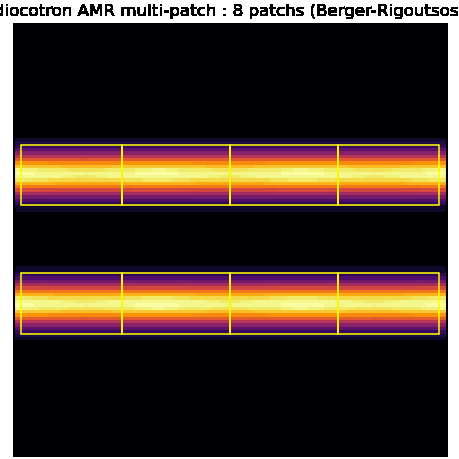
\includegraphics[width=0.48\linewidth]{multipatch_00.png}
      \hfill
      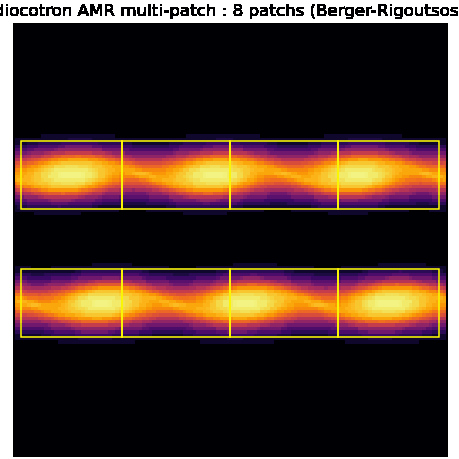
\includegraphics[width=0.48\linewidth]{multipatch_30.png}

      \vspace{0.2cm}
      \begin{block}{Critère}
        Le critère de raffinement est physique. L'infrastructure AMR est générique.
      \end{block}
    \end{column}
  \end{columns}
\end{frame}

\section{Parallélisation}

\begin{frame}[fragile]{Frontière d'exécution : \texttt{for\_each\_cell}}
\begin{lstlisting}[style=cppslide]
template <class F>
void for_each_cell(const Box2D& b, F f) {
#if defined(ADC_HAS_KOKKOS)
  Kokkos::parallel_for(
      "adc_for_each_cell",
      Kokkos::MDRangePolicy<Kokkos::Rank<2>, Kokkos::IndexType<int>>(
          {b.lo[0], b.lo[1]}, {b.hi[0] + 1, b.hi[1] + 1}),
      f);
#elif defined(_OPENMP)
  const long n_cells = long(b.hi[0] - b.lo[0] + 1) *
                       long(b.hi[1] - b.lo[1] + 1);
#pragma omp parallel for collapse(2) schedule(static) if (n_cells >= 4096)
  for (int j = b.lo[1]; j <= b.hi[1]; ++j)
    for (int i = b.lo[0]; i <= b.hi[0]; ++i) f(i, j);
#else
  for (int j = b.lo[1]; j <= b.hi[1]; ++j)
    for (int i = b.lo[0]; i <= b.hi[0]; ++i) f(i, j);
#endif
}
\end{lstlisting}
  \src{include/adc/mesh/for_each.hpp}
\end{frame}

\begin{frame}{MPI : distribution par patchs}
  \begin{columns}[T,onlytextwidth]
    \begin{column}{0.50\textwidth}
      \textbf{Structures}
      \begin{itemize}
        \item \code{DistributionMapping(nboxes,nranks)} : round-robin par défaut ;
        \item \code{parallel\_copy} : copie inter-patchs et inter-rangs ;
        \item \code{fill\_boundary} : halos intra-niveau ;
        \item \code{all\_reduce\_*} : diagnostics et registres AMR.
      \end{itemize}
    \end{column}
    \begin{column}{0.46\textwidth}
      \begin{block}{Politique niveau 0}
        \code{AmrCouplerMP} supporte un grossier répliqué par rang, ou un grossier multi-box distribué. Le répliqué reste le défaut pour les cas ROMEO testés.
      \end{block}
      \src{include/adc/parallel/comm.hpp}
    \end{column}
  \end{columns}

  \vspace{0.25cm}
  Tests MPI : chemins AMR multi-patch bit-identiques pour \(np=1,2,4\) sur les tests dédiés.
\end{frame}

\begin{frame}[fragile]{GPU : Kokkos/CUDA sans réécrire les opérateurs}
  \begin{columns}[T,onlytextwidth]
    \begin{column}{0.49\textwidth}
      \textbf{Conditions dans le code}
      \begin{itemize}
        \item lambdas \code{ADC\_HD} ;
        \item captures POD : \code{Array4}, \code{ConstArray4}, scalaires ;
        \item pas de polymorphisme dynamique dans les kernels ;
        \item \code{device\_fence()} avant lecture hôte.
      \end{itemize}
    \end{column}
    \begin{column}{0.49\textwidth}
      \textbf{CMake}
\begin{lstlisting}[style=bashslide]
cmake -B build-gpu -DADC_USE_KOKKOS=ON \
  -DCMAKE_CXX_COMPILER=$K/bin/nvcc_wrapper \
  -DKokkos_ROOT=$K
\end{lstlisting}
      \textbf{Exemples}
      \begin{itemize}
        \item \code{examples/gpu/diocotron\_amr\_kokkos.cpp}
        \item \code{examples/gpu/diocotron\_amr\_mpi\_kokkos.cpp}
      \end{itemize}
    \end{column}
  \end{columns}
\end{frame}

\begin{frame}{Mesures backend}
  \begin{columns}[T,onlytextwidth]
    \begin{column}{0.48\textwidth}
      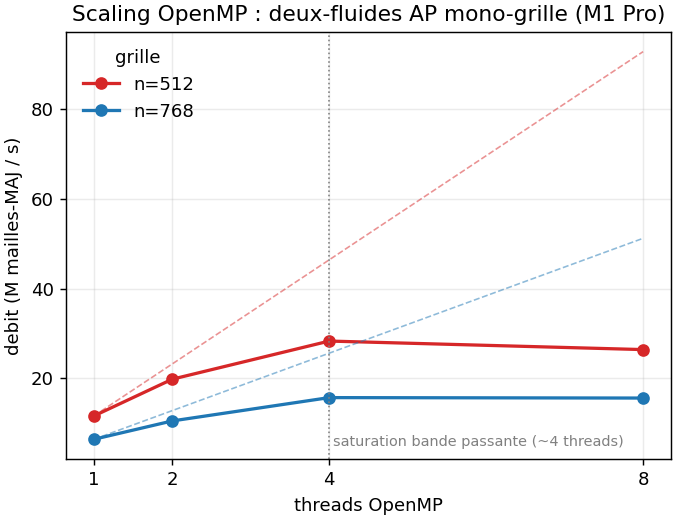
\includegraphics[width=\linewidth,height=0.58\textheight,keepaspectratio]{fig_openmp_scaling.png}
    \end{column}
    \begin{column}{0.49\textwidth}
      \textbf{Observations mesurées}
      \begin{itemize}
        \item Pas Euler--Poisson : temps dominé par Poisson.
        \item \code{OncePerStepCoupling} : \(52.3\to19.8\) ms/pas sur M1 Pro.
        \item FFT périodique : \(76\to16\) ms/pas sur Euler--Poisson.
        \item OpenMP utile seulement si le grain est suffisant ; sinon le coût de fork/join domine.
      \end{itemize}
      \vspace{0.1cm}
      \src{docs/PERFORMANCE.md}
    \end{column}
  \end{columns}
\end{frame}

\section{Construire un solveur avec \texttt{adc}}

\begin{frame}[fragile]{Étape 1 : écrire le modèle physique}
\begin{lstlisting}[style=cppslide]
struct MyModel {
  using State = adc::StateVec<N>;
  using Aux   = adc::Aux;
  static constexpr int n_vars = N;

  ADC_HD State flux(const State& u, const Aux& a, int dir) const;
  ADC_HD Real max_wave_speed(const State& u, const Aux& a, int dir) const;
  ADC_HD State source(const State& u, const Aux& a) const;
  ADC_HD Real elliptic_rhs(const State& u) const;
};

static_assert(adc::PhysicalModel<MyModel>);
\end{lstlisting}

  \vspace{0.25cm}
  Règles pratiques : fonctions locales, types POD, pas d'allocation ni \code{std::function}
  dans les formules appelées en kernel.
\end{frame}

\begin{frame}[fragile]{Étape 2 : grille uniforme couplée}
\begin{lstlisting}[style=cppslide]
adc::Box2D dom = adc::Box2D::from_extents(n, n);
adc::Geometry geom{dom, 0.0, L, 0.0, L};
adc::BoxArray ba({dom});
adc::DistributionMapping dm(ba.size(), adc::n_ranks());
adc::MultiFab U(ba, dm, MyModel::n_vars, /*ngrow=*/2);

MyModel model{/*parametres*/};
adc::BCRec bcU, bcPhi;
adc::Coupler<MyModel, adc::GeometricMG> sim(model, geom, ba, bcU, bcPhi);

for (int s = 0; s < nsteps; ++s)
  sim.advance<adc::VanLeer>(U, dt);
\end{lstlisting}

  \vspace{0.25cm}
  Variante périodique rapide : remplacer \code{GeometricMG} par un backend FFT conforme
  à \code{EllipticSolver}, quand les hypothèses FFT sont vérifiées.
\end{frame}

\begin{frame}[fragile]{Étape 3 : AMR}
\begin{lstlisting}[style=cppslide]
std::vector<adc::AmrLevelMP> levels;
levels.push_back({std::move(U0), nullptr, dx0, dy0});
levels.push_back({std::move(U1), nullptr, dx0/2, dy0/2});

adc::AmrCouplerMP<MyModel> sim(model, geom, ba0, bc, std::move(levels));

auto crit = [&](const adc::ConstArray4& u, int i, int j) {
  return indicator(u, i, j) > threshold;
};

for (int s = 0; s < nsteps; ++s) {
  if (s % 20 == 0) sim.regrid(crit);
  sim.step(dt);       // sync_down + Poisson + injection aux + advance_amr
}
\end{lstlisting}

  \vspace{0.25cm}
  L'utilisateur choisit le critère. ADC fournit clustering, nesting, interpolation,
  sous-cyclage, average-down et reflux.
\end{frame}

\begin{frame}[fragile]{Étape 4 : MPI et GPU}
  \begin{columns}[T,onlytextwidth]
    \begin{column}{0.51\textwidth}
      \textbf{MPI}
\begin{lstlisting}[style=bashslide]
cmake -B build-mpi -DADC_USE_MPI=ON
cmake --build build-mpi
mpirun -np 4 ./build-mpi/bin/diocotron_mpi out 512 600
\end{lstlisting}
      \begin{itemize}
        \item appeler \code{comm\_init} au début du \code{main} ;
        \item distribuer par \code{DistributionMapping} ;
        \item garder les diagnostics via \code{all\_reduce\_*}.
      \end{itemize}
    \end{column}
    \begin{column}{0.46\textwidth}
      \textbf{GPU}
\begin{lstlisting}[style=bashslide]
cmake -B build-gpu -DADC_USE_KOKKOS=ON \
  -DCMAKE_CXX_COMPILER=$K/bin/nvcc_wrapper \
  -DKokkos_ROOT=$K
cmake --build build-gpu
\end{lstlisting}
      Le modèle ne change pas. Les fonctions appelées dans les boucles doivent rester
      \code{ADC\_HD} et device-safe.
    \end{column}
  \end{columns}
\end{frame}

\section{ROMEO}

\begin{frame}{ROMEO : exécutions réalisées}
  \small
  \begin{tabular}{@{}p{0.16\textwidth}p{0.29\textwidth}p{0.45\textwidth}@{}}
  \toprule
  \textbf{Job} & \textbf{Configuration} & \textbf{Résultat exploitable} \\
  \midrule
  613961 & WENO5-Z + SSPRK3, modes \(3,4,5\), eff. 256--1024 &
  runs stables ; croissance mesurée, \(R^2=1.00\). \\
  613945 & colonne diocotron, NoSlope/VanLeer/AMR, eff. 512--1024 &
  AMR VanLeer suit l'uniforme avec environ \(40\%\) des cellules. \\
  614089 & GH200, Kokkos/CUDA, compute-sanitizer &
  memcheck/initcheck/synccheck sans erreur ; checksum CPU/GPU identique. \\
  614125 & convergence \(l=3,4,5\), fenêtre linéaire \([3,9]\) &
  mode 3 exact, mode 4 proche, mode 5 biaisé : effet géométrique probable. \\
  \bottomrule
  \end{tabular}

  \vspace{0.35cm}
  \src{romeo/HERO_RESULTS.md, romeo/CONV_RESULTS.md}
\end{frame}

\begin{frame}{ROMEO : AMR vs uniforme}
  \begin{columns}[T,onlytextwidth]
    \begin{column}{0.48\textwidth}
      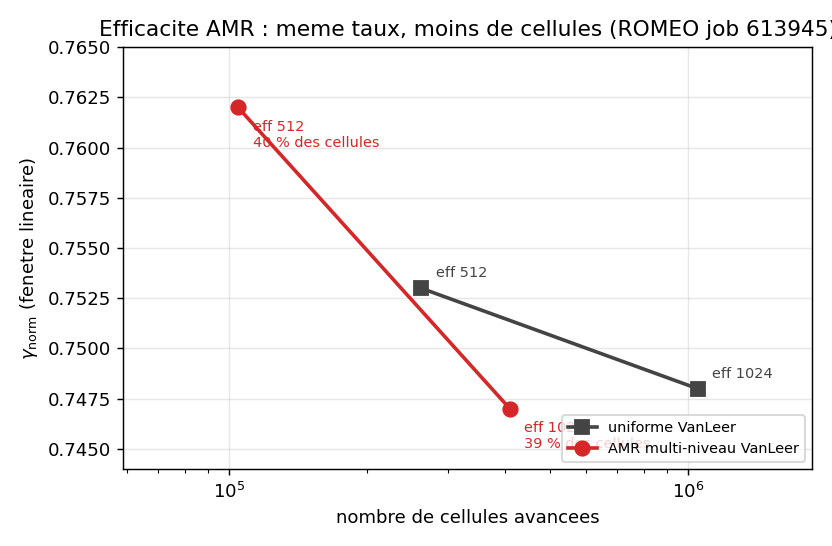
\includegraphics[width=\linewidth,height=0.55\textheight,keepaspectratio]{romeo_amr_efficiency.png}
    \end{column}
    \begin{column}{0.50\textwidth}
      \small
      \begin{tabular}{@{}lrr@{}}
      \toprule
      \textbf{Cas} & \textbf{Cellules} & \(\gamma_{\rm lin}\) \\
      \midrule
      uniforme VanLeer 512 & 262144 & 0.753 \\
      AMR VanLeer 512 & 104632 & 0.762 \\
      uniforme VanLeer 1024 & 1048576 & 0.748 \\
      AMR VanLeer 1024 & 409008 & 0.747 \\
      \bottomrule
      \end{tabular}

      \vspace{0.35cm}
      Résultat : l'AMR reproduit le taux uniforme à résolution effective identique,
      avec moins de la moitié des cellules.
    \end{column}
  \end{columns}
\end{frame}

\begin{frame}{ROMEO : taux de croissance diocotron}
  \begin{columns}[T,onlytextwidth]
    \begin{column}{0.58\textwidth}
      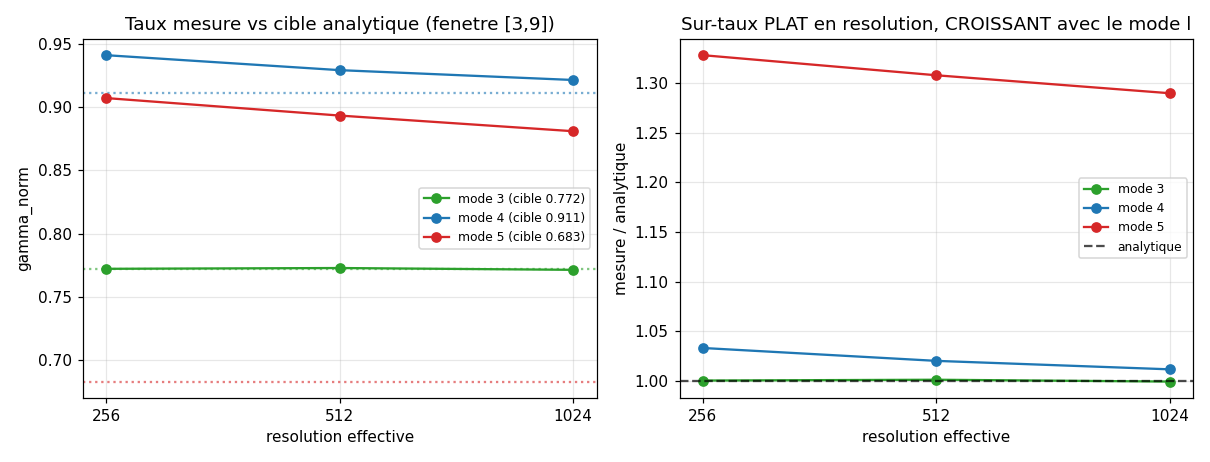
\includegraphics[width=\linewidth,height=0.60\textheight,keepaspectratio]{fig_diocotron_conv_modes.png}
    \end{column}
    \begin{column}{0.39\textwidth}
      \small
      \begin{tabular}{@{}lrr@{}}
      \toprule
      \textbf{Mode} & \textbf{cible} & \textbf{eff. 1024} \\
      \midrule
      \(l=3\) & 0.772 & 0.771 \\
      \(l=4\) & 0.911 & 0.921 \\
      \(l=5\) & 0.683 & 0.881 \\
      \bottomrule
      \end{tabular}

      \vspace{0.35cm}
      Le biais ne décroît pas avec le raffinement intérieur. L'hypothèse actuelle
      est une erreur géométrique sur la représentation cartésienne de l'anneau,
      plus marquée aux hauts modes.
    \end{column}
  \end{columns}
\end{frame}

\begin{frame}{ROMEO : validation GPU}
  \begin{columns}[T,onlytextwidth]
    \begin{column}{0.48\textwidth}
      \textbf{Job 614089, GH200}
      \begin{itemize}
        \item build Kokkos/CUDA validé ;
        \item \code{coupled\_kokkos} : memcheck, initcheck, synccheck sans erreur ;
        \item \code{diocotron\_amr\_kokkos} : memcheck sans erreur ;
        \item checksum \code{4394594.404318}, identique CPU/GPU ;
        \item dérive de masse \(2.22\times10^{-16}\).
      \end{itemize}
    \end{column}
    \begin{column}{0.48\textwidth}
      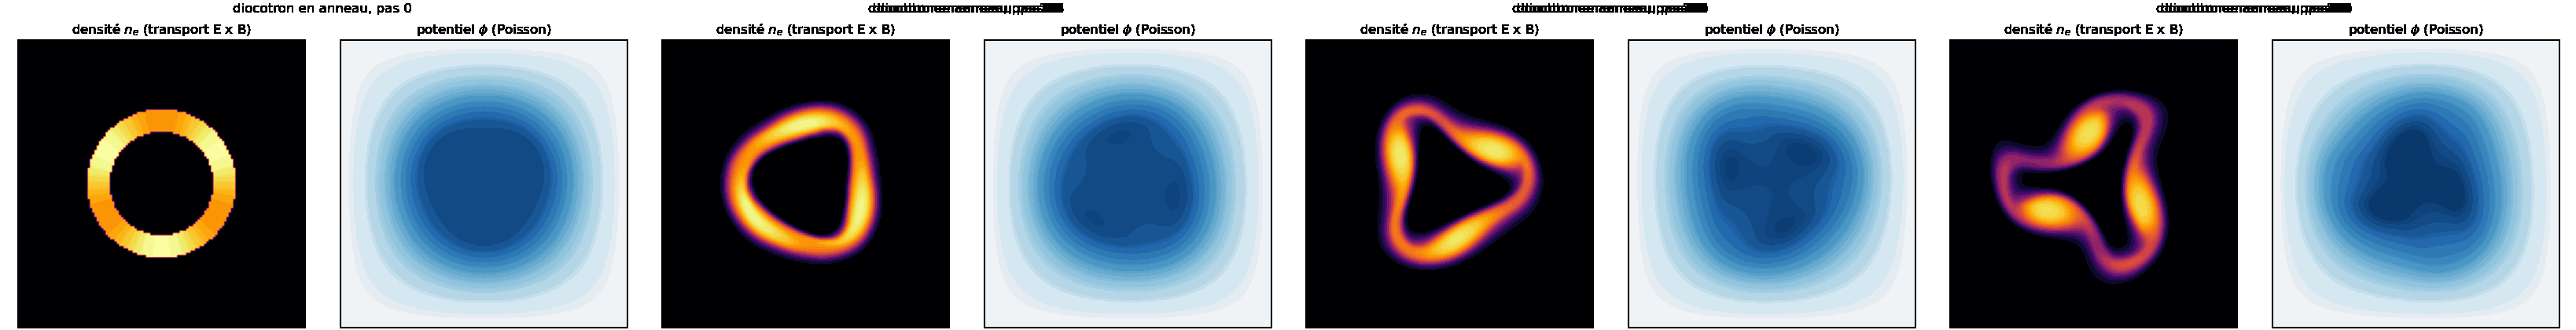
\includegraphics[width=\linewidth,height=0.55\textheight,keepaspectratio]{diocotron_ring_sequence.png}

      \vspace{0.15cm}
      {\scriptsize Exemple de run diocotron anneau ; le test GPU valide surtout la discipline mémoire et les fences.}
    \end{column}
  \end{columns}
\end{frame}

\begin{frame}{Points techniques restants}
  \begin{columns}[T,onlytextwidth]
    \begin{column}{0.49\textwidth}
      \textbf{Numérique}
      \begin{itemize}
        \item cut-cell ou level-set sur les bords \(r_0,r_1\) de l'anneau ;
        \item comparaison grille polaire pour isoler l'erreur géométrique ;
        \item extension des opérateurs elliptiques à coefficients variables.
      \end{itemize}
    \end{column}
    \begin{column}{0.49\textwidth}
      \textbf{HPC}
      \begin{itemize}
        \item load balancing SFC/knapsack pour AMR multi-patch ;
        \item tagging distribué sur niveau intermédiaire pour AMR \(3+\) niveaux ;
        \item choix automatique grossier répliqué vs distribué ;
        \item séparation éventuelle des cibles \code{adc\_serial}, \code{adc\_mpi}, \code{adc\_kokkos}.
      \end{itemize}
    \end{column}
  \end{columns}
\end{frame}

\begin{frame}{Messages techniques à défendre}
  \begin{enumerate}
    \item Le contrat \code{PhysicalModel} isole la physique des choix AMR/MPI/GPU.
    \item \code{assemble\_rhs}, \code{Coupler} et \code{advance\_amr} forment trois frontières séparées : opérateur spatial, couplage elliptique, hiérarchie AMR.
    \item L'AMR est conservatif par flux de face, average-down et reflux coverage-aware.
    \item La parallélisation n'est pas injectée dans les modèles : elle passe par \code{for\_each\_cell}, \code{DistributionMapping} et \code{comm}.
    \item Les runs ROMEO valident à la fois la physique diocotron, l'équivalence AMR/uniforme et la portabilité Kokkos/CUDA.
  \end{enumerate}
\end{frame}

\end{document}
